\documentclass{article}

\usepackage[utf8]{inputenc}
\usepackage{comment}
\usepackage{todonotes}
\usepackage{msc5}
\usepackage{listings}
\usepackage{url}
\usepackage{tikz-qtree}
\usepackage{graphicx}
\usepackage{paralist}
\usepackage{algorithm,algorithmic}
\usepackage{amsmath, amssymb, amsthm, amsfonts, caption, stmaryrd, mathtools, syntax, mdframed}
\usepackage{cryptocode}
\usepackage{hyperref}
\hypersetup{
    colorlinks,
    citecolor=black,
    filecolor=black,
    linkcolor=black,
    urlcolor=black
}

\newenvironment{prog}{\begin{array}[t]{@{}l@{}}}{\end{array}}

\theoremstyle{definition}
\newtheorem{theorem}{Theorem}[section]

\newcommand{\kwl}[1]{\mathbf{#1}}
\newcommand{\kwf}[1]{\mathsf{#1}}
\newcommand{\kwc}[1]{\mathsf{#1}}
\newcommand{\kwp}[1]{\mathsf{#1}}
\newcommand{\kwt}[1]{\mathsf{#1}}
\newcommand{\kwe}[1]{\mathsf{#1}}
\newcommand{\kwtable}[1]{\mathsf{#1}}
\newcommand{\var}[1]{\mathit{#1}}

\newcommand{\adv}{{\sf Adv}}
\newcommand{\madv}{\mathsf{Adv}}
\newcommand{\CSess}{\mathcal{C}}
\newcommand{\SSess}{\mathcal{S}}
\newcommand{\laction}[2]{$\begin{array}{c}\mbox{\textrm{#1}}\\#2\end{array}$}
\newcommand{\Z}{\mathbb{Z}}
\newcommand{\Zp}{\mathbb{Z}_p}
\newcommand{\M}{\mathbb{M}}
\newcommand{\SIGN}{\mathsf{SIGN}}
\newcommand{\HMAC}{\mathsf{HMAC}}
\newcommand{\HKDF}{\mathsf{HKDF}}
\newcommand{\ENC}{\mathsf{ENC}}
\newcommand{\DEC}{\mathsf{DEC}}
\newcommand{\sk}[1]{\mathit{sk}_{#1}}
\newcommand{\vk}[1]{\mathit{vk}_{#1}}
\newcommand{\shared}{\mathit{shared}}
\newcommand{\const}{\mathit{const}}
\newcommand{\e}{\mathit{enc}}
\newcommand{\m}{\mathit{mac}}
\newcommand{\rk}{\mathit{rk}}
\newcommand{\ck}{\mathit{ck}}
\newcommand{\tg}{\mathit{tag}}
\def\hash#1{\mathsf{H}(#1)}
\def\sign#1#2{\mathsf{sign}^{#2}(#1)}
\def\hmac#1#2{\mathsf{HMAC\mbox{-}H}^{#2}(#1)}
\def\mac#1#2{\mathsf{mac}^{#2}(#1)}
\def\tlsmac#1#2{\mathsf{mac}_{96}(#2,#1)}
\def\aead#1#2#3{\mathsf{aead}^{#2}(#1)}
\def\aenc#1#2{\mathsf{enc}^{#2}(#1)}
\def\adec#1#2{\mathsf{dec}^{#2}(#1)}
\def\mac#1#2{\mathsf{mac}^{#2}(#1)}
\def\kdf#1{\mathsf{KDF}(#1)}
\def\kdfpair#1#2{\mathsf{KDF}(#1, #2)}
\def\kdfcontext#1#2{\mathsf{KDF}(#1,#2)}
\def\dh#1#2{\mathsf{DH}(#1,#2)}
\def\kdfi#1#2{\mathsf{kdf}_{#1}(#2)}
\def\kdfz{\mathsf{kdf}_0}
\def\hkdf#1{\mathsf{hkdf}(#1)}
\def\dlog#1{\mathsf{dlog}(#1)}
\def\factor#1{\mathsf{factor}(#1)}
\def\cert{\mathit{cert}}
\def\kex{\mathit{kex}}
\def\pk{\mathit{pk}}
\def\sk{\mathit{sk}}
\def\pkp#1{\mathit{pk}_#1}
\def\skp#1{\mathit{sk}_#1}
\def\vd#1#2{\mathsf{finished}(#2,#1)}
\def\anon{\mathtt{anon}}
\def\pms{\mathit{pms}}
\def\keys{\mathit{keys}}
\def\log{\mathit{log}}
\def\ctx{\mathit{ctx}}
\def\ms{\mathit{ms}}
\def\cvd{\mathit{cvd}}
\def\svd{\mathit{svd}}
\def\sid{\mathit{sid}}
\def\mod{\mathbin{\mathrm{mod}}}
\def\info{\mathit{info}}
\def\cfg{\mathit{cfg}}
\def\nego{\mathit{nego}}
\def\uid{\mathit{uid}}
\def\pref{\mathit{Nego}}
\def\cid{\mathit{cid}}
\def\ems{\mathit{ems}}
\def\psk{\mathit{psk}}
\def\ctx{\mathit{ctx}}
\def\hk{\mathit{hk}}
\def\dk{\mathit{dk}}
\def\ak{\mathit{ak}}
\def\sni{\mathit{sni}}
\def\ksni{g^s}
\def\ksnipriv{s}

\def\seal#1#2#3#4{\mathsf{AEADEncrypt}(#1,#2,#3,#4)}
\def\open#1#2#3#4{\mathsf{AEADDecrypt}(#1,#2,#3,#4)}

\def\pch{\mathsf{CH}_{\mathsf{priv}}}
\def\esni{\mathsf{esni}}
\def\esnikey{\mathtt{'esni key'}}
\def\esniiv{\mathtt{'esni iv'}}
\def\esnibinder{\mathtt{'esni binder'}}
\def\esninonce{\mathtt{'esni nonce'}}

\theoremstyle{definition}
\newtheorem{definition}{Definition}[section]

\title{Formal Analysis of Encrypted SNI}
\author{No Name}
\date{\today}

\begin{document}

\maketitle

\begin{comment}
# Outline
- ESNI use cases, overview, and desired security goals:
    - Use cases:
        - Name privacy (coupled with DNS) against "active" attacker (modulo traffic analysis), local service discovery
    - Operational requirements and criteria: (listed from the draft)
    - Design overview:
        - Summary of draft 4
        - Overview of related designs
    - Four security/privacy requirements:
        - ESNI privacy (requirement #2):
            1. Both endpoints agree on the context
            2. Agreement implies knowledge of SNI and key share
            3. Client has proof that server has private ESNI key
    - Passive attacker: 
        - Probabilistic public key encryption (is sufficient?)
    - Known active attacks and observations:
        - Probing (client offline, draft 4): Differences in service configurations can leak information.
        - HRR mix and match (client offline, draft 4): Attacker-chosen key share, client-chosen SNI.
        - Server reaction attack (client offline, draft 4): Use ticket and server reaction for dictionary attack.
        - Client reaction attacks (earlier draft, client online): Include nonce so that same entity which sent certificate actually processed the ESNI value.
        <!-- - HRR trial decryption (client offline): Client-chosen SNI, server-chosen key share. -->
        <!-- - PSK and ENSI (draft 4): Change CH ESNI value to be attacker-controlled, and server aborts or not based on SNI+PSK equality -->
- Basic anonymous DH model (handshake secret integrity):
    - (Challenge response with the nonce)
    - Two messages (CH, SH), and proof
    - Four messages (CH1, HRR, CH2, SH), and proof
- Handshake side channels
    - (Data about handshake message size distribution?)
    - (Application data side channels -- defer to future work?)
    - CH and SH generation functions and requirements
- Integration with TLS
    - Proxy-based transformation
    - PSK binder and key schedule injection
    - (Signalling via SH.Random or explicit SH extension)
- Implementation and experimentation
\end{comment}

\begin{comment}
# Notes
- Assume that application data transfer leaks nothing about the service.

bindings: cast in terms of contexts (transcripts)
Backward binding: integrity for ClientHello
Forward binding: 
- want to detect deletion of SNI
- proxy needs DH secrets to determine the right transcript -- can't be two entities on the client side
- could treat origin padding as a configuration
- GeneraetSH must be done at the proxy, and not based on origin servers. Can get away with unmodified servers (modulo template)
- GeneraetCH/SH are the baseline properties -- show that adding forward/backward binding keeps existing properties while giving new properties
  - These may be determined by checkboxes. If any two F's are the same, then the privacy properties hold.
  - Q: should ACME be issuing certificates of a certain length

- flipping bits in CH should cause handshake keys to differ (Kazuho's does NOT do this, and there's an oracle at the client handshake)
- always need backwards binding (for messages, but possibly based on the entire transcript?)
- kazuho: enumerate domains and trial decrypt based on all possible transcripts

What we want to hide:
- SNI value itself
- A connection negotiated ESNI
- Whether the ESNI capability
- Whether the client offered ESNI

Requirements:
1. TLS agrees on SNI (forward binding, native to TLS)
2. TLS+ESNI gives us (1) and protects SNI privacy (backward binding)
  - 1/k anonymity, without forward secrecy

Optional:
3. TLS+ESNI gives (1-2) and protects the fact that ESNI was chosen
4. TLS+ESNI (1-3), plus whether the client offered ESNI


%%% Agenda:
%** Writeup review
%** ProVerif basic model with attacks -- should the ServerHello have a signal?
%** Writeup of how Kazuho/Steven PRs satisfy the basic model
%** Game-based definition (port)
\end{comment}

\tableofcontents

\section{Introduction}

The TLS Server Name Indication extension \cite{rfc6066} is an increasingly important part of the TLS protocol.
Modern TLS server deployments often offer multiple certificates behind a single IP address. The SNI helps
servers choose which certificate to choose for a given connection. However, this extension also leaks the 
server name to any on-path observer. With recent pushes to encrypt DNS and protect names from such adversaries,
the SNI extension is a privacy problem for clients. The Encrypted SNI extension \cite{ietf-tls-esni-04} attempts
to address this privacy problem by encrypting the SNI in transit. However, to date, asserting correctness and
privacy properties of the protocol proved difficult. 

\textbf{Core Protocol.} We capture the essence of ESNI in a \emph{core protocol}, which is a simplified variant
of TLS that models TLS up to the receipt of the certificate message.

\textbf{Formal Analysis.} We develop and present a ProVerif model of the core ESNI protocol to show that it
achieves the desired secrecy and privacy properties.  ProVerif analyzes symbolic protocol models using 
processes to represent entities which communicate using messages sent over public channels. Processes
can trigger security events representing attacks or critical steps of the target protocol, e.g., TLS connection establishment.
Moreover, processes can save messages in lookup tables for use later on. This is useful for storing long-term keying
material, such as ESNI and certificate private keys. Extensions to account for server reaction attacks 
(see Section \ref{sec:security}) are described, though not modeled, as there are multiple ways to build 
this property into the protocol. All models and code can be found online at \url{https://github.com/chris-wood/reftls}.

\textbf{Game-Based Analysis.} We define a game-based definition of ESNI security to complement the symbolic model.

\section{Encrypted SNI Overview}

%% XXX: misconfigurations where use of public name goes to a server that does not negotiate ESNI but does offer a certificate that terminates to the public name
%% XXX: draw figures of deployment scenarios

Encrypted SNI is a tool for hiding server names from network connections. There are several operational goals 
for Encrypted SNI \cite{requirements}, described below:
%
\begin{compactitem}
  \item Avoid widely-deployed shared secrets: One approach to the problem would be for all
  clients and servers to share a secret that encrypts (and decrypts) the SNI. However, any 
  client in this set of trusted peers could then decrypt the SNI of others. Moreover, compromise
  of any node in possession of the secret puts all members at risk. Thus, ESNI requires 
  public key encryption.
  \item Work with non-ESNI servers to avoid fallback: Without the need for fallback, ESNI 
  is a simple ECIES-like protocol, wherein the SNI is encrypted under a public key of the 
  service provider.
  \item Do not introduce extra round trips: Encrypting the SNI must not come at the cost of 
  extra round trips. For example, one possible approach is to SNI-based certificate authentication
  at the application protocol layer, e.g., using HTTP/2 Secondary Certificates \cite{ietf-httpbis-http2-secondary-certs-04}, after
  the TLS connection finishes and is authenticated with a ``public name.'' While this may work,
  the extra latency cost may be prohibitively expensive for certain clients.
  \item Forward secrecy: Ideally, SNI encryption would have some amount of forward secrecy.
  However, as SNI encryption cannot introduce additional round trips, forward secrecy is not
  possible using public key encryption primitives such as ECIES \cite{shoup2001proposal} or HPKE \cite{irtf-cfrg-hpke-00}
  \item Prevent SNI-based DoS attacks: A consequence of using public key encryption is that
  servers must perform a public key operation without having validated the client. HelloRetryRequests
  may help dampen the effects of DoS attacks, though these come at the cost of introducing
  additional complexity into the protocol. See Section \ref{sec:security} for more details.
  \item Mitigate replay attacks: Encrypted SNI values must not be replayable from one 
  ClientHello to another, otherwise an attacker could use an ESNI value from a victim client
  message in its own ClientHello.
  \item Support shared and split mode: Client-facing servers which use the SNI to determine 
  the target service may not be the entity which terminates the TLS connection. ESNI should therefore
  support proxies which route TLS connections to backend or origin services. This suggests two
  possible deployment models for ESNI, referred to as shared and split mode, as described in
  \cite{ietf-tls-esni-04}.
  %\item Do not stick out: 
  %\item Proper security context: 
  %\item Split server spoofing:
\end{compactitem}
%


% \begin{figure}
% \begin{minipage}[c]{.45\textwidth}
% \center
% 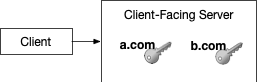
\includegraphics[scale=0.5]{esni_modes_shared.png}
% \end{minipage}
% \begin{minipage}[c]{.45\textwidth}
% \center
% 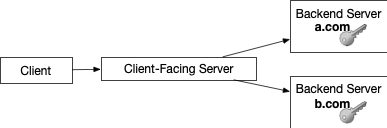
\includegraphics[scale=0.5]{esni_modes_split.png}
% \end{minipage}
% \caption{fig:modes}
% \label{Left: shared mode. Right: split mode.}
% \end{figure}

\subsection{Security and Privacy Goals} \label{sec:security}
ESNI assumes a standard active and on-path Dolev-Yao attacker that can arbitrarily drop, tamper, 
replay, and forward messages from clients. Fundamentally, a TLS handshake that negotiates ESNI should 
leak no more information than one which did not negotiate ESNI in the presence of this adversary. 
This means there are at least two necessary requirements for ESNI:
%
\begin{enumerate}
  \item SNI agreement: A successful TLS handshake implies agreement on the SNI transmitted. This means, among 
  other things, that the client authenticated the server's certificate using the SNI, and that both client and 
  server share the same view of the SNI negotiated.
  \item SNI privacy: A successful TLS handshake that negotiates ESNI does so without leaking any information 
  about the underlying SNI. Moreover, the SNI is known only to the client and server (or any recipient of the
  private ESNI key). We do not require forward secrecy for the SNI encryption.
\end{enumerate}
%
We may optionally want to hide the fact that ESNI was negotiated, as per the ``do not stick out'' goal. However, 
this is primarily only deployment concern. Furthermore, we may also want to hide the fact that a client offered
ESNI in its handshake. This may be useful for clients that wish to GREASE \cite{ietf-tls-grease-04} the extension.

\subsection{Draft-04 Design Overview and Known Attacks} \label{sec:known-attacks}
Figure \ref{fig:draft4} shows the ESNI design in draft-04 of the protocol. 

\begin{figure}[th!]
\begin{center}
\resizebox{0.8\columnwidth}{!}{\begin{msc}{}
  \drawframe{none}
  \setlength{\topheaddist}{0cm}
  \setlength{\instdist}{8.5cm}
  \setlength{\instwidth}{1.75cm}
  \declinst{cl}{}{Client $C$}
  \declinst{sr}{}{Server $S$}
  \action*{$\mathit{Knows}\ \sni, \ksni, \psk$}{cl}
  \action*{$\mathit{Knows}\ \ksnipriv, (\skp{S},\pkp{S}), \psk$}{sr}
  \nextlevel[2]
  \nextlevel
  \mess{\emph{Client Flight} ($S, g^x, \mathsf{Enc}(K_s, (r, \sni))$)}{cl}{sr}
  \nextlevel[2]
  \action*{\laction{Derive Keys:}{
    ss = \dh{g^y}{g^x} \\
    k = \kdfcontext{ss}{"esni"}}}{sr}
  \nextlevel[5]
  \mess{\emph{Server Flight} ($g^y,\mathsf{enc}(k, r)$)}{sr}{cl}
  \nextlevel
  \action*{\laction{Derive ESNI Keys:}{
    ss = \dh{g^x}{g^y} \\
    k = \kdfcontext{ss}{"esni"}}}{cl}
  \nextlevel[3]
  \end{msc}
}
\end{center}
\caption{Simple ESNI Protocol without resumption or HelloRetryRequest support.}
\label{fig:draft4}
\end{figure}

Early versions of ESNI did not achieve the desired security and privacy goals. 
For example, the first version was vulnerable to a certificate-based 
client reaction attack shown in Figure \ref{fig:attack1-client-reaction}. The SNI leak
occurs if clients processed the certificate message before verifying the CertificateVerify
signature. Specifically, if clients abort upon SNI mismatch between what they sent
and what was received in the certificate, an attacker attempt to MITM an ESNI connection
with a certificate of its choosing and try to learn the client's SNI.
The core problem was that servers did not signal to clients whether or not they processed 
the ESNI extension. Adding a nonce to the server's response implicitly authenticates
that the server processed the SNI.

\begin{figure}[th!]
\begin{center}
\resizebox{0.8\columnwidth}{!}{\begin{msc}{}
  \drawframe{none}
  \setlength{\topheaddist}{0cm}
  \setlength{\instdist}{8.5cm}
  \setlength{\instwidth}{1.75cm}
  \declinst{cl}{}{Client $C$}
  \declinst{sr}{}{Server $S$}
  \action*{$\mathit{Knows}\ \sni, \ksni$}{cl}
  \action*{$\mathit{Knows}\ \ksnipriv, (\skp{S},\pkp{S})$}{sr}
  \nextlevel[2]
  \nextlevel
  \mess{\emph{Client Flight} ($S, g^x, \mathsf{Enc}(K_s, \sni)$)}{cl}{sr}
  \nextlevel[2]
  \mess{\emph{Server Flight} ($g^y,\mathsf{enc}(k, \cert, ...), $)}{sr}{cl}
  \nextlevel
  \action*{\laction{Check SNI:}{
    \text{Abort if } \sni \text{ does not match } \cert}}{cl}
  \nextlevel[3]
  \end{msc}
}
\end{center}
\caption{Simple ESNI Protocol without resumption or HelloRetryRequest support.}
\label{fig:draft4}
\end{figure}
%

Despite this fix, draft-04 of ESNI does not achieve the necessary requirements stated above. We
describe some more attacks on ESNI deployment configurations and the protocol below.

\textbf{Probing Attacks}. If an operator partitions its servers based on SNI-specific values observable
on the wire, such as supported ciphersuites, key exchange algorithms, or application-layer protocols,
an adversary can use these differences to learn information about the client's SNI.

\textbf{HelloRetryRequest Mix and Match}. In the event of a HelloRetryRequest, clients send a fresh
key share and ESNI extension in the second ClientHello. Servers are expected to use the ESNI value
from the same ClientHello from which it received the client key shares. However, a server may use
mix and match these values, e.g., by selecting the ESNI value from the first ClientHello and the key
shares from the second ClientHello.\footnote{This is not entirely far-fetched, as some operators must
process the SNI upon the first ClientHello in order to determine HelloRetryRequest parameters such
as supported ciphersuites.} This allows an on-path adversary to hijack a HelloRetryRequest, send a
second ClientHello with its own key shares, and then successfully decrypt the server flight to learn
the certificate.

\textbf{Server Ticket Reaction Attacks}. The ESNI contents are not fully bound to the entire 
ClientHello in draft-04. This means a ClientHello with ESNI \emph{and} no resumption PSK can be 
intercepted by an on-path adversary, who then attaches a ticket and PSK binder of its choosing,
and forwards the result to the original target server. If servers check whether or not the SNI
obtained from the ESNI value and the ticket match and change behavior accordingly, e.g.,
by aborting the connection, this introduces an oracle for adversaries to learn information about
client SNIs.

In general, the problems above seem to stem from the same problems: (1) ESNI contents are not
fully bound to the ClientHello, and (2) ESNI contents are not fully bound to the rest of the TLS
handshake. In the following section, we describe an ideal ESNI protocol that addresses these
shortcomings.

\section{Core Protocol} \label{sec:core} % Basic anonymous DH model (handshake secret integrity)

At its core, ESNI is a protocol between a client and server that aims to provide the following guarantees:
%
\begin{itemize}
  \item {\bf Client Secrecy}. TLS handshake secret known by entity which has the private handshake key 
  share (y), corresponding PSK, private ESNI decryption key, and ENSI nonce. 
  \item {\bf Server Secrecy}. TLS handshake secret known by entity which has the private handshake key 
  share (x), corresponding PSK, and ENSI nonce.
  \item {\bf Agreement}. Client and server both agree on the same TLS handshake secret and transcript.
\end{itemize}
%

Thus, the core protocol only models the handshake \emph{up to the point of certificate receipt}. It does
not capture the full TLS handshake. Moreover, the core protocol does not account for server reaction
attacks, such as the one described in Section \ref{sec:security}. We treat cryptographic mitigation
of this to an extension of the core protocol. To support HelloRetryRequest flows, we also introduce a 
function $\mathsf{GenerateHRR}$ which produces a HelloRetryRequest message $\mathsf{HRR}$ given a 
ClientHello $\mathsf{CH}$.

Beyond these core protocol goals, it must also be the case that observable information, which includes 
messages sent on the wire and the \emph{actions} of clients and servers using ESNI, does not leak information
about the SNI. Indeed, the reaction attack described above was due in part to such an information 
leak.\footnote{Fortunately, backward binding resolves this problem by removing a branch in the way servers
handle ClientHello messages.} We must capture this notion of information indistinguishability for completeness.
We do so via \emph{message indistinguishability} and \emph{action indistinguishability}. Informally, message 
indistinguishability means that all messages written on the wire do not vary based on SNI. Similarly, action
indistinguishability means that all node behavior as observed by \adv\ does not vary based on SNI (or any SNI-influenced
value used in the protocol). 

We do not currently model message indistinguishability. This is because it is mainly determined by configuration.
For example, if a service provider partitions its names based on support ciphersuites, then ciphersuite
selection may leak information about the SNI. (This also applies to clients, which may, in theory, use different
ciphersuites, parameters, or extensions per domains.) Essentially, message indistinguishability requires that
all parameter selection \emph{within} the same anonymity set is SNI-agnostic.

There are two variants of the core protocol. One keeps the \emph{key schedule} secret, and another
keeps the \emph{transcript} secret. We model both in Section \ref{sec:model} and show they achieve
the desired goals. We describe them in the following subsections. The ProVerif ProVerif \cite{blanchet2016modeling} 
model used to assert their correctness is also included. Note that our models do not account for message 
indistinguishability, as this is something largely determined by configuration. 

\subsection{Key Schedule Secrecy Variant}

\begin{figure}[th!]
\begin{center}
\resizebox{0.8\columnwidth}{!}{\begin{msc}{}
  \drawframe{none}
  \setlength{\topheaddist}{0cm}
  \setlength{\instdist}{8.5cm}
  \setlength{\instwidth}{1.75cm}
  \declinst{cl}{}{Client $C$}
  \declinst{sr}{}{Server $S$}
  \action*{$\mathit{Knows}\ \sni, \ksni$}{cl}
  \action*{$\mathit{Knows}\ \ksnipriv, (\skp{S},\pkp{S})$}{sr}
  \nextlevel[2]
  \action*{\laction{Computes:}{
    x \gets \Zp, r \gets \{0,1\}^{32} \\
    \mathsf{CH} = (g^x, S, \esni = \mathsf{HPKESeal}(\ksni, (r, \sni))}}{cl}
  \nextlevel[4]
  \mess{$\mathsf{CH}$}{cl}{sr}
  \nextlevel[1]
  \action*{\laction{Computes:}{
    \mathsf{HRR} = \mathsf{GenerateHRR}(\mathsf{CH})}}{sr}
  \nextlevel[3]
  \mess{$\mathsf{HRR}$}{sr}{cl}
  \nextlevel[1]
  % \msccomment{start}{cl}
  % \nextlevel[1]
  \action*{\laction{Computes:}{
    x' \gets \Zp \\
    \mathsf{CH}' = (g^{x'}, S, \esni)}}{cl}
  \nextlevel[4]
  \mess{$\mathsf{CH}'$}{cl}{sr}
  \nextlevel[1]
  \action*{\laction{Computes:}{
    y \gets \Zp \\
    (r', \sni') = \mathsf{HPKEOpen}(\ksnipriv, \esni)) \\
    ss = \dh{g^y}{g^{x'}} \\
    k' = \kdfpair{ss}{r} \\
    k = \kdfcontext{k'}{\mathtt{'handshake secret'}} \\
    \mathsf{SH} = (g^y, \mathsf{Cert} = \seal{k}{...}{...}{\cert(\sni)})}}{sr}
  \nextlevel[8]
  \mess{$\mathsf{SH}, \mathsf{Cert}$}{sr}{cl}
  \nextlevel[1]
  \action*{\laction{Verifies:}{
    ss = \dh{g^x}{g^y} \\
    k' = \kdfpair{ss}{r} \\
    k = \kdfcontext{ss}{\mathtt{'handshake secret'}} \\ 
    \cert'(\sni') = \open{k}{...}{...}{\mathsf{Cert}}) \\
    \mathsf{Equal}(\sni', \sni)}}{cl}
  \nextlevel[6]
  \end{msc}
}
\end{center}
\caption{Minimal Core ESNI Protocol with key schedule secrecy.}
\label{fig:simple-esni-1}
\end{figure}

This core protocol variant achieves what we call \emph{forward binding} of the handshake to the ESNI 
shared secret, even in the event of HRR. Forward binding ensures the client and server secrecy
properties previously described. Note that the core protocol as described achieves this by mixing
the ESNI nonce into the TLS key schedule. Alternative designs that have the same effect exist,
and are discussed later in Section \ref{sec:proposals}.

As a consequence of forward binding and the need to interoperate with ESNI-incapable servers, 
we also require a signalling mechanism for clients to determine whether or not the ESNI contents were 
used to protect the handshake secret. (Trial decryption is always an option, though other more practical 
solutions exist.)

This core protocol variant is \emph{not} secure against server reaction attacks.
Specifically, it allows an on-path adversary to tamper with a ClientHello with no
binder in flight. Recall that the ticket-based server reaction attack relies on servers
behaving differently if the ESNI contents do not match that of the ticket contents.
In general, though, this type of reaction attack is possible in all cases where a server
performs SNI-specific behavior on unauthenticated fields in the ClientHello. 

There are at least two ways to mitigate this problem:
%
\begin{itemize}
  \item Require that servers not implement any SNI-specific check on unauthenticated fields
  in the ClientHello. This requires no protocol change, yet may be fragile in practice.
  \item Use ESNI to authenticate the entire ClientHello. This requires a protocol change.
\end{itemize}
%

For safety reasons, the second option seems prudent. Thus, to mitigate server reaction attacks,
we require the ESNI contents to authenticate the ClientHello, or to be backward bound to the 
handshake. ESNI contents are \emph{backward bound} to a ClientHello if it is not possible 
to modify a ClientHello in any way without causing an ESNI check to fail. This modification includes,
among other things, the addition of a PSK binder where one was previously not present.

The ProVerif model for this variant is below.

\begin{tabbing}
$\kwl{event}\ \kwe{ESNIClientDone}(\kwt{bitstring}, \var{element}, \var{pubkey}). $\\
$\kwl{event}\ \kwe{ESNIClientLeak}(\kwt{bitstring}, \var{element}, \var{pubkey}). $\\
$\kwl{event}\ \kwe{ESNIServerLeak}(\kwt{bitstring}, \var{element}, \kwt{bitstring}). $\\
$\kwl{event}\ \kwe{ESNIServerDone}(\kwt{bitstring}, \var{element}, \var{pubkey}). $\\
$ $\\
$\kwl{let}\ \var{ClientESNICoreHRR}() =  $\\
$\ \ \ \ \ \kwl{in}(\var{io}, (\var{host}{:}\var{prin}, \var{origin{\_}host}{:}\var{prin})); $\\
$\ \ \ \ \ \kwl{get}\ \var{esniKeys}( = \var{host},  = \var{StrongDH}, \var{xxx}, \var{gs})\ \kwl{in} $\\
$\ \ \ \ \ \kwl{let}\ \var{g} = \var{StrongDH}\ \kwl{in} $\\
$\ \ \ \ \ \kwl{let}\ \var{sni} = \var{secret{\_}sni}(\var{origin{\_}host})\ \kwl{in} $\\
$ $\\
$\ \ \ \ \ \textit{(* Derive handshake keying material *)} $\\
$\ \ \ \ \ \kwl{new}\ \var{cr}{:}\var{random}; $\\
$\ \ \ \ \ \kwl{let}\ (\var{x}{:}\kwt{bitstring}, \var{gx}{:}\var{element}) = \var{dh{\_}keygen}(\var{g})\ \kwl{in} $\\
$ $\\
$\ \ \ \ \ \textit{(* Compute HPKE(g{\string^}s, (sni{\_}nonce, sni)) *)} $\\
$\ \ \ \ \ \kwl{new}\ \var{sni{\_}nonce}{:}\var{random}; $\\
$\ \ \ \ \ \kwl{let}\ (\var{c}{:}\kwt{bitstring}, \var{gc}{:}\var{element}) = \var{dh{\_}keygen}(\var{g})\ \kwl{in} $\\
$\ \ \ \ \ \kwl{let}\ \var{gcs} = \var{e2b}(\var{dh{\_}exp}(\var{g}, \var{gs}, \var{c}))\ \kwl{in} $\\
$\ \ \ \ \ \kwl{let}\ \var{kcs} = \var{hkdf{\_}extract}(\var{zero}, \var{gcs})\ \kwl{in} $\\
$\ \ \ \ \ \kwl{let}\ \var{aek} = \var{hkdf{\_}expand{\_}label}(\var{kcs}, \var{tls13{\_}esni{\_}key}, \var{zero})\ \kwl{in} $\\
$\ \ \ \ \ \kwl{let}\ \var{aeiv} = \var{hkdf{\_}expand{\_}label}(\var{kcs}, \var{tls13{\_}esni{\_}iv}, \var{zero})\ \kwl{in} $\\
$ $\\
$\ \ \ \ \ \textit{(* Derive ESNI keying material *)} $\\
$\ \ \ \ \ \kwl{let}\ \var{esni{\_}payload} = (\var{sni{\_}nonce}, \var{sni})\ \kwl{in} $\\
$\ \ \ \ \ \kwl{let}\ \var{enc{\_}sni} = \var{aead{\_}enc}(\var{StrongAE}, \var{b2ae}(\var{aek}), \var{aeiv}, \var{zero}, \var{esni{\_}payload})\ \kwl{in} $\\
$ $\\
$\ \ \ \ \ \textit{(* The SNI extension carries the "public name", which is modeled }$\\
$\textit{        here as the public key share of the public name *)} $\\
$\ \ \ \ \ \kwl{let}\ \var{sni{\_}ext} = \var{SNI}(\var{e2b}(\var{gs}))\ \kwl{in} $\\
$ $\\
$\ \ \ \ \ \textit{(* The ESNI extension carries the the client's ESNI key share}$\\
$\textit{        and the encrypted SNI payload *)} $\\
$\ \ \ \ \ \kwl{let}\ \var{esni{\_}ext} = \var{ESNI}(\var{g}, \var{gc}, \var{enc{\_}sni})\ \kwl{in} $\\
$ $\\
$\ \ \ \ \ \textit{(* Write out the CH and get a HRR in response *)} $\\
$\ \ \ \ \ \kwl{let}\ \var{ch} = (\var{cr}, \var{gx}, \var{sni{\_}ext}, \var{esni{\_}ext})\ \kwl{in} $\\
$\ \ \ \ \ \kwl{out}(\var{io}, \var{ch}); $\\
$ $\\
$\ \ \ \ \ \kwl{in}\ (\var{io}, (\var{hrr}{:}\kwt{bitstring})); $\\
$ $\\
$\ \ \ \ \ \textit{(* Generate a new CH with a fresh key share but same ESNI contents. *)} $\\
$\ \ \ \ \ \kwl{let}\ (\var{x}{:}\kwt{bitstring}, \var{gx}{:}\var{element}) = \var{dh{\_}keygen}(\var{g})\ \kwl{in} $\\
$\ \ \ \ \ \kwl{let}\ \var{ch'} = (\var{cr}, \var{gx}, \var{sni{\_}ext}, \var{esni{\_}ext})\ \kwl{in} $\\
$\ \ \ \ \ \kwl{out}(\var{io}, \var{ch'}); $\\
$ $\\
$\ \ \ \ \ \textit{(* Read the server flight *)} $\\
$\ \ \ \ \ \kwl{in}\ (\var{io}, (\var{gy}{:}\var{element}, \var{msg}{:}\kwt{bitstring})); $\\
$ $\\
$\ \ \ \ \ \kwl{if}\ \var{gy}\neq\var{BadElement}\ \kwl{then} $\\
$\ \ \ \ \ \kwl{let}\ \var{log} = (\var{ch}, \var{hrr}, \var{ch'}, \var{gy})\ \kwl{in} $\\
$\ \ \ \ \ \kwl{let}\ \var{gxy} = \var{e2b}(\var{dh{\_}exp}(\var{g}, \var{gy}, \var{x}))\ \kwl{in} $\\
$ $\\
$\ \ \ \ \ \textit{(* Derive the handshake secret as per normal. *)} $\\
$\ \ \ \ \ \kwl{let}\ \var{kxy'} = \var{hkdf{\_}extract}(\var{zero}, \var{gxy})\ \kwl{in} $\\
$ $\\
$\ \ \ \ \ \textit{(* Mix in the ESNI nonce. *)} $\\
$\ \ \ \ \ \kwl{let}\ \var{kxy} = \var{hkdf{\_}extract}(\var{kxy'}, \var{random2b}(\var{sni{\_}nonce}))\ \kwl{in} $\\
$ $\\
$\ \ \ \ \ \textit{(* Derive remaining key material. *)} $\\
$\ \ \ \ \ \kwl{let}\ \var{aek} = \var{hkdf{\_}expand{\_}label}(\var{kxy}, \var{tls13{\_}key}, \var{log})\ \kwl{in} $\\
$\ \ \ \ \ \kwl{let}\ \var{aeiv} = \var{hkdf{\_}expand{\_}label}(\var{kxy}, \var{tls13{\_}iv}, \var{log})\ \kwl{in} $\\
$ $\\
$\ \ \ \ \ \textit{(* Decrypt the server flight *)} $\\
$\ \ \ \ \ \kwl{let}\ ((\var{recv{\_}sni}{:}\kwt{bitstring}, \var{p}{:}\var{pubkey}), \var{sig}{:}\kwt{bitstring}) = \var{aead{\_}dec}(\var{StrongAE}, \var{b2ae}(\var{aek}), \var{aeiv}, \var{zero}, \var{msg})\ \kwl{in} $\\
$\ \ \ \ \ \kwl{let}\ \var{log} = (\var{log}, (\var{recv{\_}sni}, \var{p}))\ \kwl{in} $\\
$ $\\
$\ \ \ \ \ \kwl{get}\ \var{longTermKeys}( = \var{origin{\_}host}, \var{xxxx}, \var{p})\ \kwl{in} $\\
$\ \ \ \ \ \kwl{if}\ \var{recv{\_}sni} = \var{sni}\ \kwl{then}\ ( $\\
$\ \ \ \ \ \ \kwl{if}\ \var{verify}(\var{p}, \var{log}, \var{sig}) = \kwc{true}\ \kwl{then} $\\
$\ \ \ \ \ \ \ \ \ \kwl{event}\ \kwe{ESNIClientDone}(\var{sni}, \var{gs}, \var{p})) $\\
$\ \ \ \ \ \kwl{else}\ ( $\\
$\ \ \ \ \ \ \ \ \ \ \kwl{event}\ \kwe{ESNIClientLeak}(\var{sni}, \var{gs}, \var{p}); $\\
$\ \ \ \ \ \ \kwl{out}(\var{io}, \var{sni})). $\\
$ $\\
$ $\\
$\kwl{let}\ \var{ServerESNICoreHRR}() =  $\\
$\ \ \ \ \ \kwl{in}(\var{io}, \var{host}{:}\var{prin}); $\\
$\ \ \ \ \ \kwl{get}\ \var{esniKeys}( = \var{host},  = \var{StrongDH}, \var{s}, \var{gs})\ \kwl{in} $\\
$\ \ \ \ \ \kwl{get}\ \var{longTermKeys}( = \var{host}, \var{sk}, \var{p})\ \kwl{in} $\\
$\ \ \ \ \ \kwl{let}\ \var{g} = \var{StrongDH}\ \kwl{in} $\\
$ $\\
$\ \ \ \ \ \textit{(* Read in a CH. *)} $\\
$\ \ \ \ \ \kwl{in}(\var{io}, (\var{ch}{:}\kwt{bitstring})); $\\
$\ \ \ \ \ \kwl{let}\ (\var{cr}{:}\var{random}, \var{gx}{:}\var{element}, \var{sni{\_}ext}{:}\var{sni}, \var{esni}{:}\var{sni}) = \var{ch}\ \kwl{in} $\\
$ $\\
$\ \ \ \ \ \textit{(* And send a HRR in response *)} $\\
$\ \ \ \ \ \kwl{let}\ \var{hrr} = \var{zero}\ \kwl{in} $\\
$\ \ \ \ \ \kwl{out}\ (\var{io}, \var{hrr}); $\\
$\ \ \ \ \ \kwl{in}\ (\var{io}, (\var{ch'}{:}\kwt{bitstring})); $\\
$\ \ \ \ \ \kwl{let}\ (\var{cr'}{:}\var{random}, \var{gx'}{:}\var{element}, \var{sni{\_}ext'}{:}\var{sni}, \var{esni'}{:}\var{sni}) = \var{ch'}\ \kwl{in} $\\
$ $\\
$\ \ \ \ \ \textit{(* Decrypt the ESNI contents. *)} $\\
$\ \ \ \ \ \kwl{let}\ \var{ESNI}(\var{g}, \var{gc}, \var{enc{\_}sni}) = \var{esni'}\ \kwl{in} $\\
$\ \ \ \ \ \kwl{if}\ \var{gx'}\neq\var{BadElement}\ \kwl{then} $\\
$\ \ \ \ \ \kwl{if}\ \var{gc}\neq\var{BadElement}\ \kwl{then} $\\
$\ \ \ \ \ \kwl{let}\ \var{gcs} = \var{e2b}(\var{dh{\_}exp}(\var{g}, \var{gc}, \var{s}))\ \kwl{in} $\\
$\ \ \ \ \ \kwl{let}\ \var{kcs} = \var{hkdf{\_}extract}(\var{zero}, \var{gcs})\ \kwl{in} $\\
$\ \ \ \ \ \kwl{let}\ \var{aek} = \var{hkdf{\_}expand{\_}label}(\var{kcs}, \var{tls13{\_}esni{\_}key}, \var{zero})\ \kwl{in} $\\
$\ \ \ \ \ \kwl{let}\ \var{aeiv} = \var{hkdf{\_}expand{\_}label}(\var{kcs}, \var{tls13{\_}esni{\_}iv}, \var{zero})\ \kwl{in} $\\
$\ \ \ \ \ \kwl{let}\ (\var{sni{\_}nonce}{:}\var{random}, \var{sni}{:}\kwt{bitstring}) =  $\\
$\ \ \ \ \ \ \ \ \ \var{aead{\_}dec}(\var{StrongAE}, \var{b2ae}(\var{aek}), \var{aeiv}, \var{zero}, \var{enc{\_}sni})\ \kwl{in} $\\
$ $\\
$\ \ \ \ \ \kwl{let}\ \var{origin{\_}host} = \var{get{\_}host}(\var{global{\_}sni{\_}secret}(), \var{sni})\ \kwl{in} $\\
$ $\\
$\ \ \ \ \ \kwl{let}\ (\var{y}{:}\kwt{bitstring}, \var{gy}{:}\var{element}) = \var{dh{\_}keygen}(\var{g})\ \kwl{in} $\\
$\ \ \ \ \ \kwl{let}\ \var{log} = (\var{ch}, \var{hrr}, \var{ch'}, \var{gy})\ \kwl{in} $\\
$\ \ \ \ \ \kwl{let}\ \var{gxy} = \var{e2b}(\var{dh{\_}exp}(\var{g}, \var{gx'}, \var{y}))\ \kwl{in} $\\
$ $\\
$\ \ \ \ \ \textit{(* Derive the handshake secret as per normal. *)} $\\
$\ \ \ \ \ \kwl{let}\ \var{kxy'} = \var{hkdf{\_}extract}(\var{zero}, \var{gxy})\ \kwl{in} $\\
$ $\\
$\ \ \ \ \ \textit{(* Mix in the SNI nonce. *)} $\\
$\ \ \ \ \ \kwl{let}\ \var{kxy} = \var{hkdf{\_}extract}(\var{kxy'}, \var{random2b}(\var{sni{\_}nonce}))\ \kwl{in} $\\
$ $\\
$\ \ \ \ \ \textit{(* Derive remaining key material. *)} $\\
$\ \ \ \ \ \kwl{let}\ \var{aek} = \var{hkdf{\_}expand{\_}label}(\var{kxy}, \var{tls13{\_}key}, \var{log})\ \kwl{in} $\\
$\ \ \ \ \ \kwl{let}\ \var{aeiv} = \var{hkdf{\_}expand{\_}label}(\var{kxy}, \var{tls13{\_}iv}, \var{log})\ \kwl{in} $\\
$ $\\
$\ \ \ \ \ \textit{(* Encrypt the server flight, which includes the SNI (or would-be certificate) }$\\
$\textit{        and signature over the transcript. *)} $\\
$\ \ \ \ \ \kwl{let}\ \var{log} = (\var{log}, (\var{sni}, \var{p}))\ \kwl{in} $\\
$\ \ \ \ \ \kwl{let}\ \var{sig} = \var{sign}(\var{sk}, \var{log})\ \kwl{in} $\\
$\ \ \ \ \ \kwl{let}\ \var{enc{\_}sflt} = \var{aead{\_}enc}(\var{StrongAE}, \var{b2ae}(\var{aek}), \var{aeiv}, \var{zero}, ((\var{sni}, \var{p}), \var{sig}))\ \kwl{in} $\\
$\ \ \ \ \ \kwl{out}(\var{io}, (\var{gy}, \var{enc{\_}sflt})); $\\
$\ \ \ \ \ \kwl{event}\ \kwe{ESNIServerDone}(\var{sni}, \var{gs}, \var{p}). $\\
$ $\\
$\kwl{query}\ \var{h}{:}\kwt{bitstring}, \var{gs}{:}\var{element}, \var{p}{:}\var{pubkey}; $\\
$\ \ \ \ \ \ \kwl{event}(\kwe{ESNIClientDone}(\var{h}, \var{gs}, \var{p})); $\\
$\ \ \ \ \ \ \kwl{event}(\kwe{ESNIServerDone}(\var{h}, \var{gs}, \var{p})). $\\
$ $\\
$\kwl{query}\ \var{origin{\_}host}{:}\var{prin}, \var{h}{:}\kwt{bitstring}, \var{gs}{:}\var{element}, \var{p}{:}\var{pubkey}, \var{tkt}{:}\kwt{bitstring}; $\\
$\ \ \ \ \ \ \var{attacker}(\var{secret{\_}sni}(\var{origin{\_}host})); $\\
$\ \ \ \ \ \ \kwl{event}(\kwe{ESNIClientLeak}(\var{h}, \var{gs}, \var{p})); $\\
$\ \ \ \ \ \ \kwl{event}(\kwe{ESNIServerLeak}(\var{h}, \var{gs}, \var{tkt})). $\\
$ $\\
$\textit{(* query log:bitstring; event(Reachable(log)). *)} $\\
$ $\\
$\kwl{const}\ \kwc{C}{:}\var{prin}. $\\
$\kwl{process} $\\
$\ \ \ \ \ \kwl{new}\ \var{keyA}{:}\var{ae{\_}key}; $\\
$\ \ \ \ \ \kwl{new}\ \var{keyB}{:}\var{ae{\_}key}; $\\
$\ \ \ \ \ !\var{ClientESNICoreHRR}()\mid!\var{ServerESNICoreHRR}()\mid!\var{LongTermKeys}() $\\
$$
\end{tabbing}

\subsection{Transcript Secrecy Variant}

\begin{figure}[th!]
\begin{center}
\resizebox{0.8\columnwidth}{!}{\begin{msc}{}
  \drawframe{none}
  \setlength{\topheaddist}{0cm}
  \setlength{\instdist}{8.5cm}
  \setlength{\instwidth}{1.75cm}
  \declinst{cl}{}{Client $C$}
  \declinst{sr}{}{Server $S$}
  \action*{$\mathit{Knows}\ \sni, \ksni$}{cl}
  \action*{$\mathit{Knows}\ \ksnipriv, (\skp{S},\pkp{S})$}{sr}
  \nextlevel[2]
  \action*{\laction{Computes:}{
    x \gets \Zp, x_p \gets \Zp \\
    \mathsf{CH}_{\mathsf{priv}} = (g^{x_p}, \sni) \\
    \mathsf{CH} = (g^x, S, \pch = \mathsf{HPKESeal}(\ksni, \mathsf{CH}_{\mathsf{priv}})}}{cl}
  \nextlevel[5]
  \mess{$\mathsf{CH}$}{cl}{sr}
  \nextlevel[1]
  \action*{\laction{Computes:}{
    \mathsf{HRR} = \mathsf{GenerateHRR}(\mathsf{CH})}}{sr}
  \nextlevel[3]
  \mess{$\mathsf{HRR}$}{sr}{cl}
  \nextlevel[1]
  % \msccomment{start}{cl}
  % \nextlevel[1]
  \action*{\laction{Computes:}{
    x' \gets \Zp \\
    \mathsf{CH}' = (g^{x'}, S, \pch)}}{cl}
  \nextlevel[4]
  \mess{$\mathsf{CH}'$}{cl}{sr}
  \nextlevel[1]
  \action*{\laction{Computes:}{
    y \gets \Zp \\
    (g^{x_p}, \sni) = \mathsf{HPKEOpen}(\ksnipriv, \pch) \\
    ss = \dh{g^y}{g^{x_p}} \\
    k = \kdfcontext{k'}{\mathtt{'handshake secret'}} \\
    \mathsf{SH} = (g^y, \mathsf{Cert} = \seal{k}{...}{...}{\cert(\sni)})}}{sr}
  \nextlevel[8]
  \mess{$\mathsf{SH}, \mathsf{Cert}$}{sr}{cl}
  \nextlevel[1]
  \action*{\laction{Verifies:}{
    ss = \dh{g^{x_p}}{g^y} \\
    k = \kdfcontext{ss}{\mathtt{'handshake secret'}} \\ 
    \cert'(\sni') = \open{k}{...}{...}{\mathsf{Cert}}) \\
    \mathsf{Equal}(\sni', \sni)}}{cl}
  \nextlevel[6]
  \end{msc}
}
\end{center}
\caption{Minimal Core ESNI Protocol with transcript secrecy.}
\label{fig:simple-esni-2}
\end{figure}

Note that this diagram does not show the flow where the server chooses the outer ``public''
ClientHello. As in the prior core protocol variant, some signalling mechanism is needed 
for clients to determine which ClientHello was used. 

Unlike the prior variant, this design \emph{does} achieve forward and backward binding by
design, since the private ClientHello is authenticated via encryption. (Note that the interaction
with session resumption is also left out. In practice, this variant might include ESNI 
resumption PSK binders only in the private ClientHello.) However, this design comes at the cost
of building handshake secrecy on secrecy of the transcript. We discuss this property in Section \ref{sec:proposals}.

The ProVerif model for this variant is below.

\begin{tabbing}
$\kwl{event}\ \kwe{ESNIClientDone}(\kwt{bitstring}, \var{element}, \var{pubkey}). $\\
$\kwl{event}\ \kwe{ESNIClientLeak}(\kwt{bitstring}, \var{element}, \var{pubkey}). $\\
$\kwl{event}\ \kwe{ESNIServerLeak}(\kwt{bitstring}, \var{element}, \kwt{bitstring}). $\\
$\kwl{event}\ \kwe{ESNIServerDone}(\kwt{bitstring}, \var{element}, \var{pubkey}). $\\
$\kwl{event}\ \kwe{ESNINonESNIServerDone}(\kwt{bitstring}, \var{element}, \var{pubkey}). $\\
$ $\\
$\kwl{let}\ \var{ClientESNICoreHRR}() =  $\\
$\ \ \ \ \ \kwl{in}(\var{io}, (\var{host}{:}\var{prin}, \var{origin{\_}host}{:}\var{prin})); $\\
$\ \ \ \ \ \kwl{get}\ \var{esniKeys}( = \var{host},  = \var{StrongDH}, \var{xxx}, \var{gs})\ \kwl{in} $\\
$\ \ \ \ \ \kwl{let}\ \var{g} = \var{StrongDH}\ \kwl{in} $\\
$\ \ \ \ \ \kwl{let}\ \var{sni} = \var{secret{\_}sni}(\var{origin{\_}host})\ \kwl{in} $\\
$ $\\
$\ \ \ \ \ \textit{(* Derive handshake keying material *)} $\\
$\ \ \ \ \ \kwl{new}\ \var{cr}{:}\var{random}; $\\
$\ \ \ \ \ \kwl{let}\ (\var{x}{:}\kwt{bitstring}, \var{gx}{:}\var{element}) = \var{dh{\_}keygen}(\var{g})\ \kwl{in} $\\
$ $\\
$\ \ \ \ \ \textit{(* Compute HPKE(g{\string^}s, (g{\string^}x, ch)) = HPKE(g{\string^}s, (g{\string^}x, (g{\string^}x', sni)))  *)} $\\
$\ \ \ \ \ \kwl{let}\ (\var{c}{:}\kwt{bitstring}, \var{gc}{:}\var{element}) = \var{dh{\_}keygen}(\var{g})\ \kwl{in} $\\
$\ \ \ \ \ \kwl{let}\ \var{gcs} = \var{e2b}(\var{dh{\_}exp}(\var{g}, \var{gs}, \var{c}))\ \kwl{in} $\\
$\ \ \ \ \ \kwl{let}\ \var{kcs} = \var{hkdf{\_}extract}(\var{zero}, \var{gcs})\ \kwl{in} $\\
$\ \ \ \ \ \kwl{let}\ \var{aek} = \var{hkdf{\_}expand{\_}label}(\var{kcs}, \var{tls13{\_}esni{\_}key}, \var{zero})\ \kwl{in} $\\
$\ \ \ \ \ \kwl{let}\ \var{aeiv} = \var{hkdf{\_}expand{\_}label}(\var{kcs}, \var{tls13{\_}esni{\_}iv}, \var{zero})\ \kwl{in} $\\
$ $\\
$\ \ \ \ \ \textit{(* Derive the private ClientHello *)} $\\
$\ \ \ \ \ \kwl{let}\ (\var{x2}{:}\kwt{bitstring}, \var{gx2}{:}\var{element}) = \var{dh{\_}keygen}(\var{g})\ \kwl{in} $\\
$\ \ \ \ \ \kwl{let}\ \var{private{\_}ch} = (\var{gx2}, \var{sni})\ \kwl{in} $\\
$\ \ \ \ \ \kwl{let}\ \var{tunnel{\_}ch} = \var{aead{\_}enc}(\var{StrongAE}, \var{b2ae}(\var{aek}), \var{aeiv}, \var{zero}, \var{private{\_}ch})\ \kwl{in} $\\
$ $\\
$\ \ \ \ \ \textit{(* The SNI extension carries the "public name", which is modeled }$\\
$\textit{        here as the public key share of the public name *)} $\\
$\ \ \ \ \ \kwl{let}\ \var{sni{\_}ext} = \var{SNI}(\var{e2b}(\var{gs}))\ \kwl{in} $\\
$ $\\
$\ \ \ \ \ \textit{(* The ESNI extension carries the the client's ESNI key share}$\\
$\textit{        and the encrypted SNI payload *)} $\\
$\ \ \ \ \ \kwl{let}\ \var{tunnel{\_}ext} = (\var{g}, \var{gc}, \var{tunnel{\_}ch})\ \kwl{in} $\\
$ $\\
$\ \ \ \ \ \textit{(* Write out the CH and get a HRR in response *)} $\\
$\ \ \ \ \ \kwl{let}\ \var{ch} = (\var{cr}, \var{gx}, \var{sni{\_}ext}, \var{tunnel{\_}ext})\ \kwl{in} $\\
$\ \ \ \ \ \kwl{out}(\var{io}, \var{ch}); $\\
$ $\\
$\ \ \ \ \ \kwl{in}\ (\var{io}, (\var{hrr}{:}\kwt{bitstring})); $\\
$ $\\
$\ \ \ \ \ \textit{(* Generate a new CH with a fresh key share but same ESNI contents. *)} $\\
$\ \ \ \ \ \kwl{let}\ (\var{x}{:}\kwt{bitstring}, \var{gx}{:}\var{element}) = \var{dh{\_}keygen}(\var{g})\ \kwl{in} $\\
$\ \ \ \ \ \kwl{let}\ \var{ch'} = (\var{cr}, \var{gx}, \var{sni{\_}ext}, \var{tunnel{\_}ext})\ \kwl{in} $\\
$\ \ \ \ \ \kwl{out}(\var{io}, \var{ch'}); $\\
$ $\\
$\ \ \ \ \ \textit{(* Read the server flight *)} $\\
$\ \ \ \ \ \kwl{in}\ (\var{io}, (\var{gy}{:}\var{element}, \var{msg}{:}\kwt{bitstring})); $\\
$ $\\
$\ \ \ \ \ \kwl{if}\ \var{gy}\neq\var{BadElement}\ \kwl{then} $\\
$ $\\
$\ \ \ \ \ \textit{(* Derive the handshake secret using the private CH *)} $\\
$\ \ \ \ \ \kwl{let}\ \var{log} = (\var{private{\_}ch}, \var{gy})\ \kwl{in} $\\
$\ \ \ \ \ \kwl{let}\ \var{gxy} = \var{e2b}(\var{dh{\_}exp}(\var{g}, \var{gy}, \var{x2}))\ \kwl{in} $\\
$\ \ \ \ \ \kwl{let}\ \var{kxy} = \var{hkdf{\_}extract}(\var{zero}, \var{gxy})\ \kwl{in} $\\
$\ \ \ \ \ \kwl{let}\ \var{aek} = \var{hkdf{\_}expand{\_}label}(\var{kxy}, \var{tls13{\_}key}, \var{log})\ \kwl{in} $\\
$\ \ \ \ \ \kwl{let}\ \var{aeiv} = \var{hkdf{\_}expand{\_}label}(\var{kxy}, \var{tls13{\_}iv}, \var{log})\ \kwl{in} $\\
$\ \ \ \ \  $\\
$\ \ \ \ \ \kwl{let}\ ((\var{recv{\_}sni}{:}\kwt{bitstring}, \var{p}{:}\var{pubkey}), \var{sig}{:}\kwt{bitstring}) = \var{aead{\_}dec}(\var{StrongAE}, \var{b2ae}(\var{aek}), \var{aeiv}, \var{zero}, \var{msg})\ \kwl{in} $\\
$\ \ \ \ \ \kwl{if}\ \var{recv{\_}sni} = \var{sni}\ \kwl{then}\ ( $\\
$\ \ \ \ \ \ \ \ \ \kwl{let}\ \var{log} = (\var{log}, (\var{recv{\_}sni}, \var{p}))\ \kwl{in} $\\
$\ \ \ \ \ \ \ \ \ \kwl{get}\ \var{longTermKeys}( = \var{origin{\_}host}, \var{xxxx}, \var{p})\ \kwl{in} $\\
$\ \ \ \ \ \ \ \ \ \kwl{if}\ \var{recv{\_}sni} = \var{sni}\ \kwl{then}\ ( $\\
$\ \ \ \ \ \ \ \ \ \ \kwl{if}\ \var{verify}(\var{p}, \var{log}, \var{sig}) = \kwc{true}\ \kwl{then} $\\
$\ \ \ \ \ \ \ \ \ \ \ \ \kwl{event}\ \kwe{ESNIClientDone}(\var{sni}, \var{gs}, \var{p})) $\\
$\ \ \ \ \ \ \ \ \ \kwl{else}\ ( $\\
$\ \ \ \ \ \ \ \ \ \ \ \ \kwl{event}\ \kwe{ESNIClientLeak}(\var{sni}, \var{gs}, \var{p}); $\\
$\ \ \ \ \ \ \ \ \ \ \ \ \kwl{out}(\var{io}, \var{sni}))) $\\
$\ \ \ \ \kwl{else}\ ( $\\
$\ \ \ \ \ \ \ \ \textit{(* Derive the handshake secret using the public CH *)} $\\
$\ \ \ \ \ \ \ \ \kwl{let}\ \var{log} = (\var{ch}, \var{gy})\ \kwl{in} $\\
$\ \ \ \ \ \ \ \ \kwl{let}\ \var{gxy} = \var{e2b}(\var{dh{\_}exp}(\var{g}, \var{gy}, \var{x}))\ \kwl{in} $\\
$\ \ \ \ \ \ \ \ \kwl{let}\ \var{kxy'} = \var{hkdf{\_}extract}(\var{zero}, \var{gxy})\ \kwl{in} $\\
$\ \ \ \ \ \ \ \ \kwl{let}\ \var{aek} = \var{hkdf{\_}expand{\_}label}(\var{kxy}, \var{tls13{\_}key}, \var{log})\ \kwl{in} $\\
$\ \ \ \ \ \ \ \ \kwl{let}\ \var{aeiv} = \var{hkdf{\_}expand{\_}label}(\var{kxy}, \var{tls13{\_}iv}, \var{log})\ \kwl{in} $\\
$\ \ \ \ \ \ \ \ \kwl{let}\ ((\var{recv{\_}sni}{:}\kwt{bitstring}, \var{p}{:}\var{pubkey}), \var{sig}{:}\kwt{bitstring}) = \var{aead{\_}dec}(\var{StrongAE}, \var{b2ae}(\var{aek}), \var{aeiv}, \var{zero}, \var{msg})\ \kwl{in} $\\
$\ \ \ \ \ \ \ \ \kwl{let}\ \var{log} = (\var{log}, (\var{recv{\_}sni}, \var{p}))\ \kwl{in} $\\
$\ \ \ \ \ \ \ \ \ \kwl{get}\ \var{longTermKeys}( = \var{origin{\_}host}, \var{xxxx}, \var{p})\ \kwl{in} $\\
$\ \ \ \ \ \ \ \ \ \kwl{if}\ \var{recv{\_}sni} = \var{sni}\ \kwl{then}\ ( $\\
$\ \ \ \ \ \ \ \ \ \ \kwl{if}\ \var{verify}(\var{p}, \var{log}, \var{sig}) = \kwc{true}\ \kwl{then} $\\
$\ \ \ \ \ \ \ \ \ \ \ \ \kwl{event}\ \kwe{ESNIClientDone}(\var{sni}, \var{gs}, \var{p})) $\\
$\ \ \ \ \ \ \ \ \ \kwl{else}\ ( $\\
$\ \ \ \ \ \ \ \ \ \ \ \ \kwl{event}\ \kwe{ESNIClientLeak}(\var{sni}, \var{gs}, \var{p}); $\\
$\ \ \ \ \ \ \ \ \ \ \ \ \kwl{out}(\var{io}, \var{sni}))). $\\
$\ \ \ \ \ \ \ \  $\\
$\kwl{let}\ \var{ServerESNICoreHRR}() =  $\\
$\ \ \ \ \ \kwl{in}(\var{io}, \var{host}{:}\var{prin}); $\\
$\ \ \ \ \ \kwl{get}\ \var{esniKeys}( = \var{host},  = \var{StrongDH}, \var{s}, \var{gs})\ \kwl{in} $\\
$\ \ \ \ \ \kwl{get}\ \var{longTermKeys}( = \var{host}, \var{sk}, \var{p})\ \kwl{in} $\\
$\ \ \ \ \ \kwl{let}\ \var{g} = \var{StrongDH}\ \kwl{in} $\\
$ $\\
$\ \ \ \ \ \textit{(* Read in a CH. *)} $\\
$\ \ \ \ \ \kwl{in}(\var{io}, (\var{ch}{:}\kwt{bitstring})); $\\
$\ \ \ \ \ \kwl{let}\ (\var{cr}{:}\var{random}, \var{gx}{:}\var{element}, \var{sni{\_}ext}{:}\var{sni}, \var{tunnel{\_}ext}{:}\kwt{bitstring}) = \var{ch}\ \kwl{in} $\\
$ $\\
$\ \ \ \ \ \textit{(* And send a HRR in response *)} $\\
$\ \ \ \ \ \kwl{let}\ \var{hrr} = \var{zero}\ \kwl{in} $\\
$\ \ \ \ \ \kwl{out}\ (\var{io}, \var{hrr}); $\\
$\ \ \ \ \ \kwl{in}\ (\var{io}, (\var{ch'}{:}\kwt{bitstring})); $\\
$\ \ \ \ \ \kwl{let}\ (\var{cr'}{:}\var{random}, \var{gx'}{:}\var{element}, \var{sni{\_}ext'}{:}\var{sni}, \var{esni'}{:}\var{sni}) = \var{ch'}\ \kwl{in} $\\
$ $\\
$\ \ \ \ \ \textit{(* Decrypt the private CH. *)} $\\
$\ \ \ \ \ \kwl{let}\ (\var{g}{:}\var{group}, \var{gc}{:}\var{element}, \var{tunnel{\_}ch}{:}\kwt{bitstring}) = \var{tunnel{\_}ext}\ \kwl{in} $\\
$\ \ \ \ \ \kwl{if}\ \var{gx'}\neq\var{BadElement}\ \kwl{then} $\\
$\ \ \ \ \ \kwl{if}\ \var{gc}\neq\var{BadElement}\ \kwl{then} $\\
$\ \ \ \ \ \kwl{let}\ \var{gcs} = \var{e2b}(\var{dh{\_}exp}(\var{g}, \var{gc}, \var{s}))\ \kwl{in} $\\
$\ \ \ \ \ \kwl{let}\ \var{kcs} = \var{hkdf{\_}extract}(\var{zero}, \var{gcs})\ \kwl{in} $\\
$\ \ \ \ \ \kwl{let}\ \var{aek} = \var{hkdf{\_}expand{\_}label}(\var{kcs}, \var{tls13{\_}esni{\_}key}, \var{zero})\ \kwl{in} $\\
$\ \ \ \ \ \kwl{let}\ \var{aeiv} = \var{hkdf{\_}expand{\_}label}(\var{kcs}, \var{tls13{\_}esni{\_}iv}, \var{zero})\ \kwl{in} $\\
$ $\\
$\ \ \ \ \ \kwl{let}\ (\var{gx2}{:}\var{element}, \var{sni}{:}\kwt{bitstring}) =  $\\
$\ \ \ \ \ \ \ \ \ \var{aead{\_}dec}(\var{StrongAE}, \var{b2ae}(\var{aek}), \var{aeiv}, \var{zero}, \var{tunnel{\_}ch})\ \kwl{in} $\\
$\ \ \ \ \ \kwl{let}\ \var{private{\_}ch} = (\var{gx2}, \var{sni})\ \kwl{in} $\\
$ $\\
$\ \ \ \ \ \kwl{let}\ \var{origin{\_}host} = \var{get{\_}host}(\var{global{\_}sni{\_}secret}(), \var{sni})\ \kwl{in} $\\
$ $\\
$\ \ \ \ \ \kwl{let}\ (\var{y}{:}\kwt{bitstring}, \var{gy}{:}\var{element}) = \var{dh{\_}keygen}(\var{g})\ \kwl{in} $\\
$\ \ \ \ \ \kwl{let}\ \var{log} = (\var{private{\_}ch}, \var{gy})\ \kwl{in} $\\
$\ \ \ \ \ \kwl{let}\ \var{gxy} = \var{e2b}(\var{dh{\_}exp}(\var{g}, \var{gx2}, \var{y}))\ \kwl{in} $\\
$ $\\
$\ \ \ \ \ \textit{(* Derive the handshake secret as per normal. *)} $\\
$\ \ \ \ \ \kwl{let}\ \var{kxy} = \var{hkdf{\_}extract}(\var{zero}, \var{gxy})\ \kwl{in} $\\
$ $\\
$\ \ \ \ \ \textit{(* Derive remaining key material. *)} $\\
$\ \ \ \ \ \kwl{let}\ \var{aek} = \var{hkdf{\_}expand{\_}label}(\var{kxy}, \var{tls13{\_}key}, \var{log})\ \kwl{in} $\\
$\ \ \ \ \ \kwl{let}\ \var{aeiv} = \var{hkdf{\_}expand{\_}label}(\var{kxy}, \var{tls13{\_}iv}, \var{log})\ \kwl{in} $\\
$ $\\
$\ \ \ \ \ \textit{(* Encrypt the server flight, which includes the SNI (or would-be certificate) }$\\
$\textit{        and signature over the transcript. *)} $\\
$\ \ \ \ \ \kwl{let}\ \var{log} = (\var{log}, (\var{sni}, \var{p}))\ \kwl{in} $\\
$\ \ \ \ \ \kwl{let}\ \var{sig} = \var{sign}(\var{sk}, \var{log})\ \kwl{in} $\\
$\ \ \ \ \ \kwl{let}\ \var{enc{\_}sflt} = \var{aead{\_}enc}(\var{StrongAE}, \var{b2ae}(\var{aek}), \var{aeiv}, \var{zero}, ((\var{sni}, \var{p}), \var{sig}))\ \kwl{in} $\\
$\ \ \ \ \ \kwl{out}(\var{io}, (\var{gy}, \var{enc{\_}sflt})); $\\
$\ \ \ \ \ \kwl{event}\ \kwe{ESNIServerDone}(\var{sni}, \var{gs}, \var{p}). $\\
$ $\\
$\kwl{let}\ \var{ServerNoESNICoreHRR}() =  $\\
$\ \ \ \ \ \kwl{in}(\var{io}, \var{host}{:}\var{prin}); $\\
$\ \ \ \ \ \kwl{get}\ \var{esniKeys}( = \var{host},  = \var{StrongDH}, \var{s}, \var{gs})\ \kwl{in} $\\
$\ \ \ \ \ \kwl{get}\ \var{longTermKeys}( = \var{host}, \var{sk}, \var{p})\ \kwl{in} $\\
$\ \ \ \ \ \kwl{let}\ \var{g} = \var{StrongDH}\ \kwl{in} $\\
$ $\\
$\ \ \ \ \ \textit{(* Read in a CH. *)} $\\
$\ \ \ \ \ \kwl{in}(\var{io}, (\var{ch}{:}\kwt{bitstring})); $\\
$\ \ \ \ \ \kwl{let}\ (\var{cr}{:}\var{random}, \var{gx}{:}\var{element}, \var{sni{\_}ext}{:}\var{sni}, \var{tunnel{\_}ext}{:}\kwt{bitstring}) = \var{ch}\ \kwl{in} $\\
$\ \ \ \ \ \kwl{let}\ \var{SNI}(\var{e2b}( = \var{gs})) = \var{sni{\_}ext}\ \kwl{in} $\\
$ $\\
$\ \ \ \ \ \kwl{let}\ (\var{y}{:}\kwt{bitstring}, \var{gy}{:}\var{element}) = \var{dh{\_}keygen}(\var{g})\ \kwl{in} $\\
$\ \ \ \ \ \kwl{let}\ \var{log} = (\var{ch}, \var{gy})\ \kwl{in} $\\
$\ \ \ \ \ \kwl{let}\ \var{gxy} = \var{e2b}(\var{dh{\_}exp}(\var{g}, \var{gx}, \var{y}))\ \kwl{in} $\\
$ $\\
$\ \ \ \ \ \textit{(* Derive the handshake secret as per normal. *)} $\\
$\ \ \ \ \ \kwl{let}\ \var{kxy} = \var{hkdf{\_}extract}(\var{zero}, \var{gxy})\ \kwl{in} $\\
$ $\\
$\ \ \ \ \ \textit{(* Derive remaining key material. *)} $\\
$\ \ \ \ \ \kwl{let}\ \var{aek} = \var{hkdf{\_}expand{\_}label}(\var{kxy}, \var{tls13{\_}key}, \var{log})\ \kwl{in} $\\
$\ \ \ \ \ \kwl{let}\ \var{aeiv} = \var{hkdf{\_}expand{\_}label}(\var{kxy}, \var{tls13{\_}iv}, \var{log})\ \kwl{in} $\\
$ $\\
$\ \ \ \ \ \textit{(* Encrypt the server flight, which includes the SNI (or would-be certificate) }$\\
$\textit{        and signature over the transcript. *)} $\\
$\ \ \ \ \ \kwl{let}\ \var{log} = (\var{log}, (\var{gs}, \var{p}))\ \kwl{in} $\\
$\ \ \ \ \ \kwl{let}\ \var{sig} = \var{sign}(\var{sk}, \var{log})\ \kwl{in} $\\
$\ \ \ \ \ \kwl{let}\ \var{enc{\_}sflt} = \var{aead{\_}enc}(\var{StrongAE}, \var{b2ae}(\var{aek}), \var{aeiv}, \var{zero}, ((\var{e2b}(\var{gs}), \var{p}), \var{sig}))\ \kwl{in} $\\
$\ \ \ \ \ \kwl{out}(\var{io}, (\var{gy}, \var{enc{\_}sflt})); $\\
$\ \ \ \ \ \kwl{event}\ \kwe{ESNINonESNIServerDone}(\var{e2b}(\var{gs}), \var{gs}, \var{p}). $\\
$ $\\
$\kwl{query}\ \var{h}{:}\kwt{bitstring}, \var{gs}{:}\var{element}, \var{p}{:}\var{pubkey}; $\\
$\ \ \ \ \ \ \kwl{event}(\kwe{ESNIClientDone}(\var{h}, \var{gs}, \var{p})); $\\
$\ \ \ \ \ \ \kwl{event}(\kwe{ESNIServerDone}(\var{h}, \var{gs}, \var{p})); $\\
$\ \ \ \ \ \ \kwl{event}(\kwe{ESNINonESNIServerDone}(\var{h}, \var{gs}, \var{p})). $\\
$ $\\
$\kwl{query}\ \var{origin{\_}host}{:}\var{prin}, \var{h}{:}\kwt{bitstring}, \var{gs}{:}\var{element}, \var{p}{:}\var{pubkey}, \var{tkt}{:}\kwt{bitstring}; $\\
$\ \ \ \ \ \ \var{attacker}(\var{secret{\_}sni}(\var{origin{\_}host})); $\\
$\ \ \ \ \ \ \kwl{event}(\kwe{ESNIClientLeak}(\var{h}, \var{gs}, \var{p})); $\\
$\ \ \ \ \ \ \kwl{event}(\kwe{ESNIServerLeak}(\var{h}, \var{gs}, \var{tkt})). $\\
$ $\\
$\textit{(* query log:bitstring; event(Reachable(log)). *)} $\\
$ $\\
$\kwl{const}\ \kwc{C}{:}\var{prin}. $\\
$\kwl{process} $\\
$\ \ \ \ \ \kwl{new}\ \var{keyA}{:}\var{ae{\_}key}; $\\
$\ \ \ \ \ \kwl{new}\ \var{keyB}{:}\var{ae{\_}key}; $\\
$\ \ \ \ \ !\var{ClientESNICoreHRR}()\mid!\var{ServerESNICoreHRR}()\mid!\var{ServerNoESNICoreHRR}()\mid!\var{LongTermKeys}() $\\
$$
\end{tabbing}

\section{Summary of Proposals} \label{sec:proposals}

There are two proposals that conform to the core ESNI protocol described in Section \ref{sec:core}. 
They are summarized below.

\textbf{ESNI Proxy Transformation}. This proposal implements the transcript secrecy core protocol variant. 
A high level summary of this proposal is as follows:
%
\begin{itemize}
  \item Bind the ESNI contents to the entire ClientHello with an explicit transformation function
  that works as follows. Given a fully-formed ``private'' ClientHello (with the unencrypted SNI 
  value and ESNI nonce), encrypt the SNI value using the ClientHello as AAD, and output a ``public'' 
  ClientHelo with the SNI extension replaced with the ESNI extension. 
  \item Bind the ESNI contents to the handshake by choosing either the ``public'' or reconstructed
  ``private'' ClientHello to mix into the transcript. 
  \item Do not send an ESNI extension in the event of HRR.
\end{itemize}
%
It has the following properties:
%
\begin{itemize}
  \item[$+$] ClientHello messages sent in response to HelloRetryRequest messages do not carry an ESNI
  extension, which means that servers must maintain state about which SNI was chosen from the first ClientHello.
  \item[$-$] The transcript used upon ESNI negotiation is not that which is sent over the wire. This is
  a significant deviation from the TLS 1.3 model and introduces interesting side effects, such as the
  ability of an unknown third party, e.g., a backend origin server, to complete the handshake without
  the client being aware. (This is a problem in TLS in general, as secret information can always be
  exfiltrated to another party to complete the handshake.)
  \item[$-$] Treats the handshake transcript, which is fed into the TLS key schedule as the {\tt Info}
  parameter to {\tt HKDF-Expand}, as secret information. (In contrast, the normal transcript in TLS 1.3
  is composed of public information.) Note that HKDF leaks no information about this parameter
  if modeled as a random oracle or if the key is secret. More generally, PRFs have no guarantees about
  the secrecy of their inputs if the key is known. Importantly, in this proposal, an attacker
  does know the key in the event of HRR, yet the input is secret. Bellare and Lysyanskaya \cite{bellare2015symmetric}
  proved that HMAC satisfies the notion of a dualPRF, which roughly states that HMAC is a PRF if 
  either the the key or the input is secret. Thus, in practice, this should not affect security, though
  it may affect the proofs used for TLS 1.3.
\end{itemize}
%

\textbf{ESNI Tunnel Transformation}. This proposal implements the transcript secrecy core protocol variant. 
A high level summary of this proposal is as follows:
%
\begin{itemize}
  \item Encrypt a fully formed ``private'' ClientHello under the server's public ESNI key. Then, include
  this encryption as an extension in an outer ``public'' ClientHello.
  \item Bind the ESNI contents to the handshake by choosing either the ``public'' or reconstructed
  ``private'' ClientHello to mix into the transcript.
\end{itemize}
%
This proposal is similar to the proxy transformation change, with the following notable differences:
%
\begin{itemize}
  \item[$+$] The private ClientHello is encrypted and authenticated, rather than simply authenticated.
  \item[$-$] The public ClientHello nearly doubles in size to store the encrypted private ClientHello.
\end{itemize}
%

\textbf{ESNI PSK Binders and Key Schedule Injection}. This proposal implements the key schedule secrecy 
core protocol variant. A high level summary of this proposal is as follows:
%
\begin{itemize}
  \item Bind the ESNI contents to the entire ClientHello with an explicit PSK binder, whose value is
  derived from the ESNI shared secret.
  \item Bind the ESNI contents to the handshake by mixing the derived ESNI nonce into the key schedule.
  \item Always generate and send an ESNI extension. In the event of HRR, the contents of this ESNI 
  extension are identical to that of the first ClientHello.
\end{itemize}
%
It has the following properties:
%
\begin{itemize}
  \item[$+$] Backward binding relies on existing PSK binder properties.
  \item[$+$] HelloRetryRequest contents do not change across ClientHello messages, simplifying server
  implementations.
  \item[$-$] Forward binding requires key schedule modification.
  \item[$-$] In the event of session resumption, two binders are added to a ClientHello and both
  must be verified by the server. This goes against text in the TLS 1.3 specification \cite{rfc8446}, 
  which states that servers ``SHOULD NOT attempt to validate multiple binders.''
\end{itemize}
%

\bibliographystyle{plain}
\bibliography{references}

\end{document}

